\section{Video RF Overlay en redes FTTH}
\label{sec:rf_overlay}

El RF Overlay distribuye televisión sobre una red FTTH superponiendo, en una longitud de onda propia, el mismo espectro de RF que circula por una red de cable: los canales de $6 \, [MHz]$ de $47$ a $1.000 \, [MHz]$. El espectro completo de la cabecera modula en intensidad un láser de $1.550 \, [nm]$, viaja por la misma fibra y los mismos divisores ópticos que los datos de la red PON, y en la casa del abonado un receptor óptico lo convierte de nuevo en la señal de RF original, que se entrega por coaxial al televisor.

Desde el punto de vista del televisor, el RF Overlay es indistinguible de una red de cable, y desde el punto de vista de la red, es un servicio de difusión pura, independiente del sistema PON de datos con el que comparte la fibra. La Recomendación G.983.3 definió una banda de mejora de $1.550$ a $1.560 \, [nm]$ para servicios de video \cite{itu_g9833}, que G.984.5 conservó para GPON \cite{itu_g9845}.

\subsection{Integración con los servicios de datos}
La red PON de datos y el RF Overlay comparten toda la red de distribución óptica (ODN), pero se separan por longitud de onda (multiplexación WDM):
\begin{itemize}
    \item \underline{En la cabecera}, un combinador WDM une la salida de video, en $1.550 \, [nm]$, con el puerto PON de la OLT, que transmite en $1.490 \, [nm]$ y recibe en $1.310 \, [nm]$.
    \item \underline{En la ODN}, la fibra troncal, los divisores ópticos y las acometidas transportan las tres longitudes de onda sin distinción: los divisores son pasivos y de banda ancha.
    \item \underline{En la casa del abonado}, un filtro WDM separa el $1.550 \, [nm]$ hacia el receptor de video y deja pasar $1.490/1.310 \, [nm]$ hacia la ONT de datos.
\end{itemize}
Los dos servicios son independientes: el video no consume capacidad de los puertos GPON, y una falla de la OLT no interrumpe la televisión ni viceversa. Lo único que comparten es la ODN, y con ella su atenuación.

\begin{figure}[H]
    \centering
    \begin{tikzpicture}[every node/.style={font=\small},
        caja/.style={draw, rounded corners, minimum height=1.15cm, minimum width=2.7cm, align=center, fill=blue!6},
        int/.style={draw, fill=white, align=center, minimum width=2.4cm, minimum height=0.8cm},
        opt/.style={very thick, red!70!black}, rf/.style={thick, blue!60!black}, dat/.style={thick, green!55!black}]
        % Fila 1: cabecera de video
        \node[caja, fill=orange!12] (fuentes) at (0, 0) {Satélite, fibra\\y señales locales};
        \node[caja] (cab) at (3.7, 0) {Cabecera RF\\(moduladores\\QAM o ISDB-Tb)};
        \node[caja] (txo) at (7.4, 0) {Transmisor óptico\\$1.550 \, nm$};
        \node[caja] (edfa) at (11.1, 0) {Amplificador\\óptico EDFA};
        % Fila 2: datos y combinación
        \node[caja, fill=orange!12] (red) at (0, -2.4) {Red IP /\\enlace mayorista};
        \node[caja] (olt) at (3.7, -2.4) {OLT GPON\\$1.490 / 1.310 \, nm$};
        \node[caja] (wdm) at (11.1, -2.4) {Combinador\\WDM};
        % Fila 3: ODN
        \node[caja] (spl) at (11.1, -4.8) {Divisores ópticos\\$1{:}4$ y $1{:}16$};
        % Fila 4: abonado
        \node[int] (rxv) at (11.1, -8.0) {Receptor de\\video $1.550$};
        \node[int] (ontd) at (11.1, -9.2) {ONT de datos};
        \node[font=\small\bfseries] (ontlab) at (11.1, -7.2) {ONT con CATV};
        \node[draw, rounded corners, fill=green!8, fit=(ontlab)(rxv)(ontd), inner sep=5pt] (ont) {};
        \node[font=\small\bfseries] at (11.1, -7.2) {ONT con CATV};
        \node[int] (rxv) at (11.1, -8.0) {Receptor de\\video $1.550$};
        \node[int] (ontd) at (11.1, -9.2) {ONT de datos};
        \node[caja, fill=yellow!12] (tv) at (6.4, -8.0) {Televisores\\(coaxial $75 \, \Omega$)};
        \node[caja, fill=yellow!12] (lan) at (6.4, -9.4) {Router, Wi-Fi\\y STB IPTV};
        % Conexiones
        \draw[-{Stealth}] (fuentes) -- (cab);
        \draw[-{Stealth}, rf] (cab) -- node[above, font=\scriptsize]{RF} (txo);
        \draw[-{Stealth}, opt] (txo) -- node[above, font=\scriptsize]{$1.550$} (edfa);
        \draw[-{Stealth}, opt] (edfa) -- (wdm);
        \draw[{Stealth}-{Stealth}, dat] (red) -- (olt);
        \draw[{Stealth}-{Stealth}, opt] (olt) -- node[above, font=\scriptsize]{$1.490 / 1.310$} (wdm);
        \draw[{Stealth}-{Stealth}, opt] (wdm) -- node[right, font=\scriptsize]{fibra troncal ($3 \, \lambda$)} (spl);
        \draw[{Stealth}-{Stealth}, opt] (spl) -- node[pos=0.4, right, font=\scriptsize]{acometida} (ont);
        \draw[-{Stealth}, rf] (rxv) -- node[above, font=\scriptsize]{RF} (tv);
        \draw[{Stealth}-{Stealth}, dat] (ontd.west) -- node[above, font=\scriptsize]{Ethernet} (lan.east |- ontd.west);
        % Agrupaciones
        \node[draw, dashed, fit=(cab)(edfa)(olt)(wdm), inner sep=8pt, label={[font=\small]above:Oficina central / cabecera}] {};
        \node[draw, dashed, fit=(spl), inner sep=8pt, label={[font=\small]left:ODN}] {};
        \node[draw, dashed, fit=(ont)(tv)(lan), inner sep=8pt, label={[font=\small]below:Domicilio del abonado}] {};
        % Leyenda
        \node[align=left, font=\scriptsize, anchor=west] at (-1.35, -6.0) {%
            \textcolor{red!70!black}{\rule[0.5ex]{0.6cm}{1.5pt}} fibra óptica\\[2pt]
            \textcolor{blue!60!black}{\rule[0.5ex]{0.6cm}{1pt}} RF (video)\\[2pt]
            \textcolor{green!55!black}{\rule[0.5ex]{0.6cm}{1pt}} datos (eléctrico)};
    \end{tikzpicture}
    \caption{Diagrama en bloques de una red FTTH con RF Overlay.}
    \label{fig:rf_overlay}
\end{figure}

\subsection{Equipos y componentes principales}
\begin{itemize}
    \item \underline{Cabecera de RF:} reúne los canales de televisión. Recibe señales satelitales y de fibra, las decodifica y las vuelve a modular en canales de $6 \, [MHz]$, en DVB-C, ISDB-Tb o PAL-N, y las combina en un único espectro de RF, igual al de una red de cable.
    \item \underline{Transmisor óptico de $1.550 \, [nm]$:} convierte ese espectro de RF en una modulación de intensidad del láser. Como lleva muchos canales a la vez, debe ser muy lineal, para que no aparezcan productos de intermodulación de segundo y tercer orden sobre otros canales.
    \item \underline{Amplificador óptico EDFA:} amplifica directamente la señal óptica de $1.550 \, [nm]$. Compensa la atenuación de la división: una ODN 1:64 atenúa unos $25 \, [dB]$. Los EDFA de video tienen muchas salidas, una por cada puerto PON.
    \item \underline{Combinador WDM:} acopla el video de $1.550 \, [nm]$ con el puerto PON en una sola fibra, con bajas pérdidas de inserción y buen aislamiento entre longitudes de onda.
    \item \underline{Red de distribución óptica:} la misma ODN de la red de datos, con la fibra troncal, los divisores y las acometidas.
    \item \underline{Receptor de video:} un fotodiodo con un amplificador de RF de bajo ruido convierte la potencia óptica en la señal de RF original.
\end{itemize}

\subsection{Longitudes de onda}
La \autoref{fig:longitudes} resume el plan de longitudes de onda habitual cuando el RF Overlay comparte la ODN con GPON y, eventualmente, con XGS-PON \cite{itu_g9845, itu_g98071}:
\begin{itemize}
    \item \underline{GPON:} $1.490 \, [nm]$ en bajada y $1.310 \, [nm]$ en subida.
    \item \underline{Video RF Overlay:} $1.550$ a $1.560 \, [nm]$, en un solo sentido.
    \item \underline{XGS-PON:} $1.577 \, [nm]$ en bajada y $1.270 \, [nm]$ en subida.
\end{itemize}

\begin{figure}[H]
    \centering
    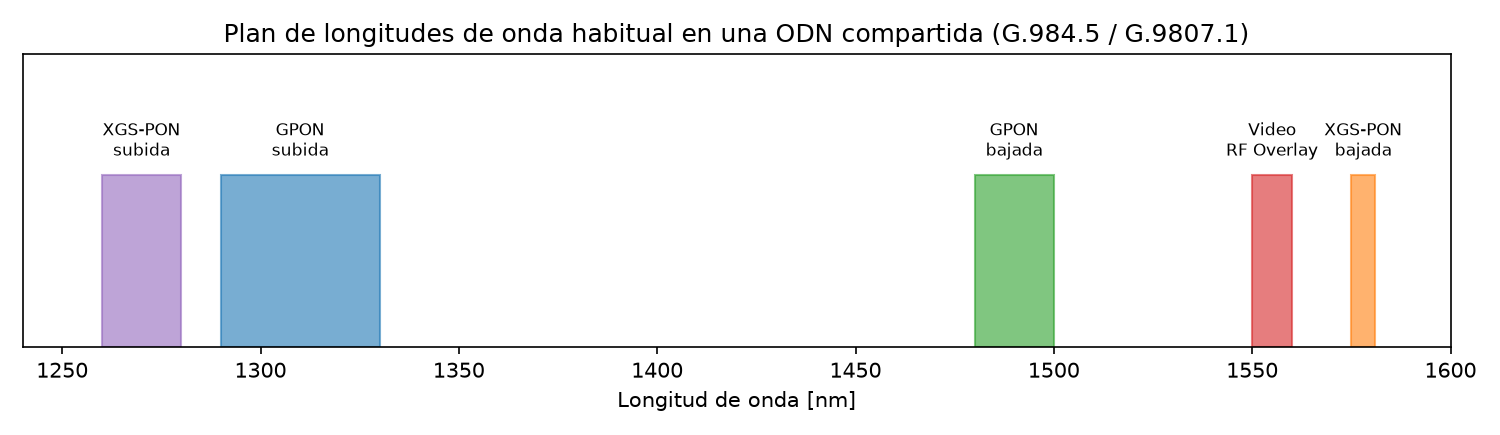
\includegraphics[width=\textwidth]{teoria/longitudes_onda.png}
    \caption{Longitudes de onda de GPON, XGS-PON y RF Overlay sobre una misma ODN.}
    \label{fig:longitudes}
\end{figure}

\subsection{Llegada de la señal al televisor}
El receptor óptico entrega por su salida coaxial el mismo espectro que sale de la cabecera. Desde allí, un cable coaxial de $75 \, [\Omega]$ (con divisores de RF si hay varios televisores) lleva la señal a cada aparato, como en una instalación de cable convencional. El televisor sintoniza los canales con su propio sintonizador: analógico PAL-N, ISDB-Tb, si la cabecera modula en esa norma, o DVB-C, si el televisor lo admite (y, si hace falta, un decodificador para canales cifrados).


\subsection{Diferencias entre RF Overlay e IPTV}
La \autoref{tab:overlay_iptv} compara ambas alternativas, con sus ventajas y limitaciones.

\begin{table}[H]
    \centering
    \small
    \caption{Comparación entre RF Overlay e IPTV en una red FTTH.}
    \label{tab:overlay_iptv}
    \renewcommand{\arraystretch}{1.2}
    \begin{tabular}{p{2.6cm} >{\raggedright\arraybackslash}p{5.9cm} >{\raggedright\arraybackslash}p{5.9cm}}
        \toprule
          & \textbf{RF Overlay} & \textbf{IPTV} \\
        \midrule
        \textbf{Transporte} & Espectro de RF completo, en modulación de intensidad a $1.550 \, [nm]$ & Paquetes IP multicast dentro del canal de datos de la PON \\
        \midrule
        \textbf{Distribución} & Difusión: los canales llegan siempre a todos los abonados & Bajo demanda: solo viajan los canales que se están mirando \\
        \midrule
        \textbf{Recepción} & Sintonizador del televisor, por coaxial & Decodificador IP (STB) o aplicación, por HDMI o Wi-Fi \\
        \midrule
        \textbf{Ventajas} &
        \begin{itemize}[nosep, leftmargin=*, before=\vspace{-0.6\baselineskip}, after=\vspace{-\baselineskip}]
            \item Los televisores existentes funcionan sin decodificador.
            \item Cada televisor de la casa sintoniza por su cuenta, sin equipos adicionales.
            \item No carga la red de datos, y el cambio de canal es tan rápido como el del sintonizador.
            \item Fácil migrar de una red HFC.
        \end{itemize} &
        \begin{itemize}[nosep, leftmargin=*, before=\vspace{-0.6\baselineskip}, after=\vspace{-\baselineskip}]
            \item Una sola red IP para todos los servicios, sin equipamiento óptico de video.
            \item Servicios interactivos: video a pedido, programación diferida y grabación en red.
            \item Cantidad de canales casi ilimitada, porque solo se transportan los que se miran.
        \end{itemize} \\
        \vspace{1pt}\\
        \midrule
        \textbf{Limitaciones} &
        \begin{itemize}[nosep, leftmargin=*, before=\vspace{-0.6\baselineskip}, after=\vspace{-\baselineskip}]
            \item Requiere equipamiento óptico de alta linealidad y potencia (transmisores, EDFA), costoso y específico para video.
            \item La CNR depende de la potencia óptica recibida, lo que exige un presupuesto óptico propio, más ajustado con canales analógicos que con digitales.
            \item Los canales pagos requieren acceso condicional en un decodificador.
        \end{itemize} &
        \begin{itemize}[nosep, leftmargin=*, before=\vspace{-0.6\baselineskip}, after=\vspace{-\baselineskip}]
            \item Necesita un STB o un televisor inteligente con aplicación por cada pantalla.
            \item Consume capacidad de los puertos PON y del enlace mayorista.
            \item Requiere una red con multicast, IGMP y calidad de servicio bien configurados.
            \item Es sensible a la congestión y a la pérdida de paquetes.
        \end{itemize} \\
        \vspace{1pt}\\
        \bottomrule
    \end{tabular}
\end{table}